%!TEX root = ../NCVC.tex

\subsection{加工条件詳細}

\subsubsection{基本}
\begin{minipage}[t]{0.5\textwidth}
 【\ref{sec:init.nci} 加工条件の設定】や【\ref{sec:init2.nci} 加工条件の設定2】を参照して下さい.
カスタムヘッダー・フッターで使用できるキーワードは \ref{sec:custom} に記載しました.
\end{minipage}
\begin{minipage}[t]{0.5\textwidth}
\vspace*{-2zh}
\begin{figure}[H]
\centering
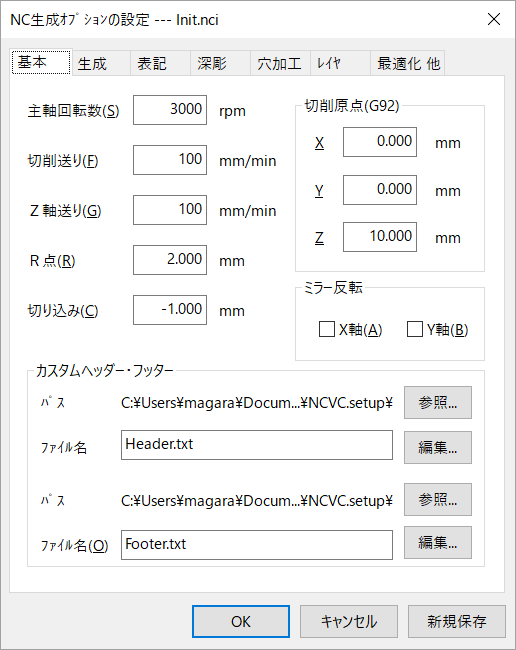
\includegraphics[scale=0.7]{No6/fig/init1.png}
\label{fig:init1.png}
\end{figure}
\end{minipage}

\subsubsection{生成}
\begin{minipage}[t]{0.5\textwidth}
 ブロック設定の[書式]はC言語のprintf命令と同じ書式で指示します.
チェック無く使用されますので,正しく指示して下さい.
[EOB 出力]は行末に ``\,;,\''(セミコロン)等が必要なときに設定します.

 位置指令の[Z軸復帰]は切削データが途切れて次のシマへ移動するときのZ軸座標を指示します.
イニシャル点かR点が選択できます.
\end{minipage}
\begin{minipage}[t]{0.5\textwidth}
\vspace*{-2zh}
\begin{figure}[H]
\centering
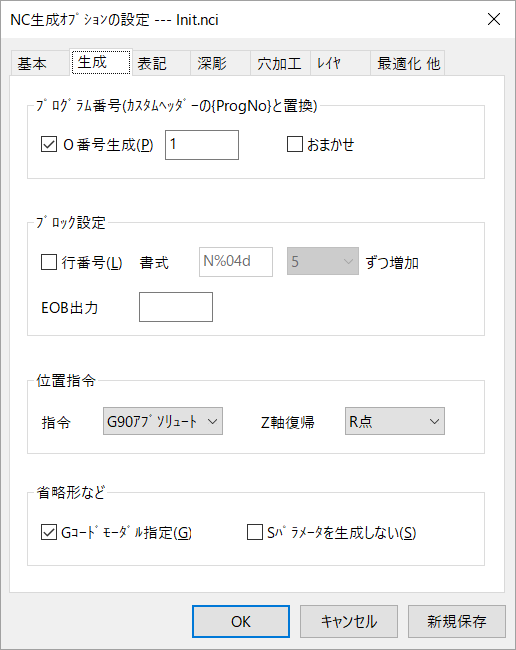
\includegraphics[scale=0.7]{No6/fig/init2.png}
\label{fig:init2.png}
\end{figure}
\end{minipage}

\subsubsection{表記}
\begin{minipage}[t]{0.5\textwidth}
 ほぼ見たままですが,ここでの注意点は数値表記の設定です.
小数点・1/1000・整数から選択できますが,座標や値をそれぞれ,そのまま(1/1000 四捨五入)・千倍・小数点以下切り捨て,で出力されます.
特にFパラメータで1以下の低速指示を行う場合,整数ではゼロになるので注意して下さい.
\end{minipage}
\begin{minipage}[t]{0.5\textwidth}
\vspace*{-2zh}
\begin{figure}[H]
\centering
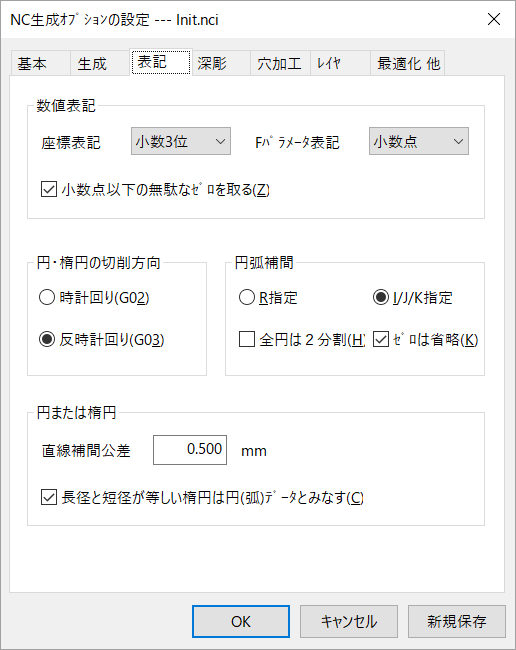
\includegraphics[scale=0.7]{No6/fig/init3.png}
\label{fig:init3.png}
\end{figure}
\end{minipage}

\subsubsection{深彫}
\begin{minipage}[t]{0.5\textwidth}
 【\ref{sec:deep} 深彫切削】も併せて参照して下さい.
[加工済み深さの指示]は,その下の[Z軸送り]速度で G01 移動させるときの指示.
加工済みであっても G00 では不安,基本タブの[Z軸送り]では遅いなどの場合に指示します.
指定は今から加工するZ値に対するオフセット,または,固定値が選択できます.
[最終Z値仕上げ]は[最終切り込み]のZ値の段階で個別に回転数や送り速度を指示する場合に使います.
\end{minipage}
\begin{minipage}[t]{0.5\textwidth}
\vspace*{-2zh}
\begin{figure}[H]
\centering
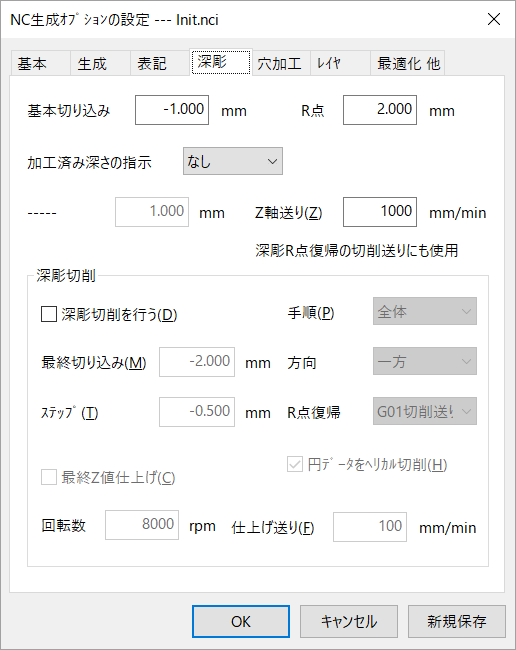
\includegraphics[scale=0.7]{No6/fig/init4.png}
\label{fig:init4.png}
\end{figure}
\end{minipage}

\subsubsection{穴加工}
\begin{minipage}[t]{0.5\textwidth}
 【\ref{sec:hole} 穴加工】も併せて参照して下さい.
[切削順序]は穴加工・軌跡加工両方のCADデータがあるとき,どちらを先に生成するかを指示します.
[穴加工のみ]では通常の切削データが生成されませんのでご注意下さい.
\end{minipage}
\begin{minipage}[t]{0.5\textwidth}
\vspace*{-2zh}
\begin{figure}[H]
\centering
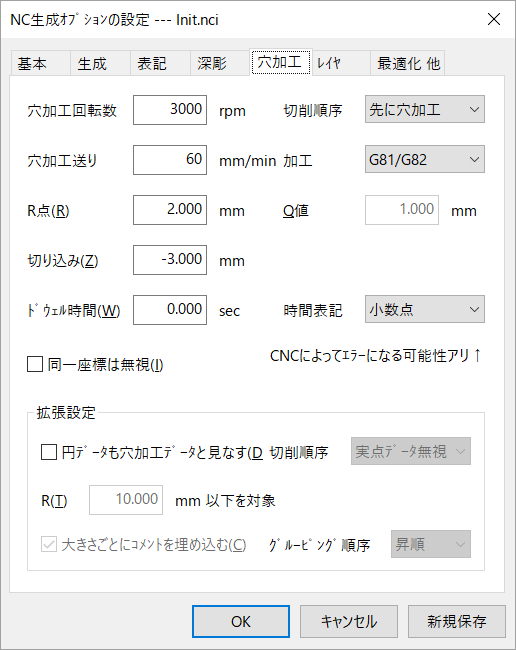
\includegraphics[scale=0.7]{No6/fig/init5.png}
\label{fig:init5.png}
\end{figure}
\end{minipage}

\subsubsection{レイヤ}
\begin{minipage}[t]{0.5\textwidth}
 【\ref{sec:multi-layer} 複数レイヤ処理】と【\ref{sec:move} 移動レイヤ】も併せて参照して下さい.
[複数レイヤごとにコメントを埋め込む]にチェックが入っていると処理するレイヤごとにコメントを自動挿入します.
単一レイヤでは挿入されません.
移動レイヤのZ値は,そのまま・R点復帰・イニシャル点復帰が選択できます.
カスタム移動コードは,移動指示のたびに挿入されるコードです.
【\ref{sec:moji} Gコードの埋め込み】では毎回必要ですが,常に特殊コードが必要な場合はこちらが便利.
ワイヤー加工機などが該当するでしょう.
\end{minipage}
\begin{minipage}[t]{0.5\textwidth}
\vspace*{-2zh}
\begin{figure}[H]
\centering
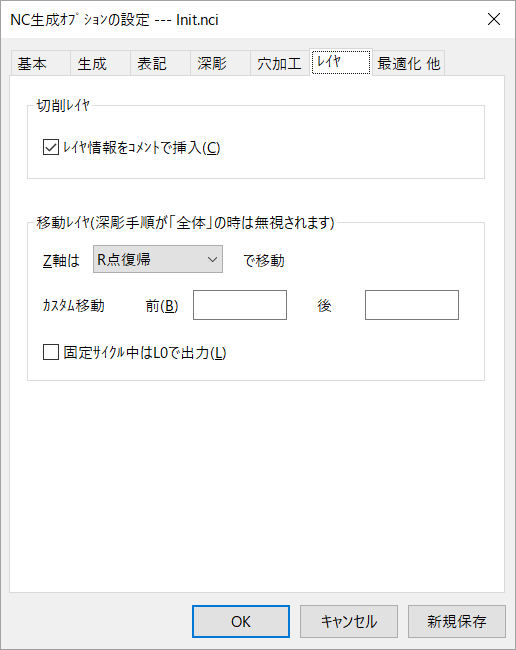
\includegraphics[scale=0.7]{No6/fig/init6.png}
\label{fig:init6.png}
\end{figure}
\end{minipage}

\subsubsection{最適化}
\begin{minipage}[t]{0.5\textwidth}
 切削データ座標検索条件では同一座標と見なす許容差を指示します.
許容差以上なら[Z軸上昇後次の切削ポイントへ移動]か[G01による補間]が選択できますが,通常は使わないで下さい.
ここで調整するよりもCADでの作図でキッチリと端点を接続する方が得策です.
穴加工データ探索の優先軸では,同一のX軸またはY軸を優先的に生成します.
優先軸なしの場合,NCVCは最短データを検索します.
\end{minipage}
\begin{minipage}[t]{0.5\textwidth}
\vspace*{-2zh}
\begin{figure}[H]
\centering
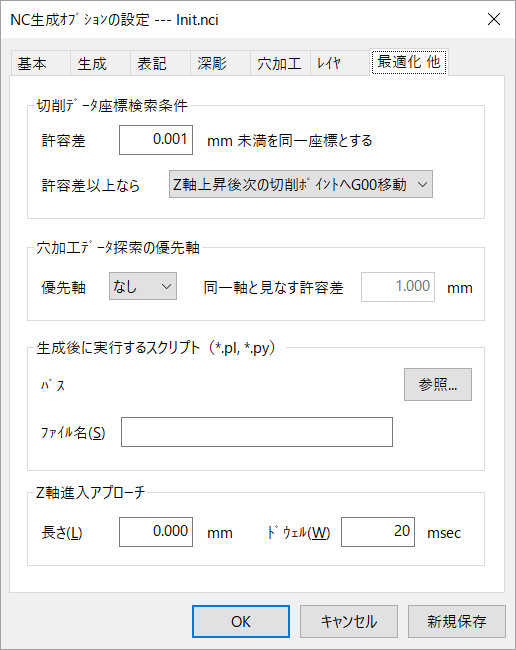
\includegraphics[scale=0.7]{No6/fig/init7.png}
\label{fig:init7.png}
\end{figure}
\end{minipage}

\subsubsection{カスタムヘッダー・フッターの置換キーワード}
 ``\,\{\,'' と ``\,\}\,'' で括られたとき置換キーワードと認識されます.

\begin{table}[H]
\centering
\begin{tabular}{|p{3cm}|p{10cm}|}
\hline
MakeDate & \smash{\raisebox{-1zh}{生成した日付と時間に置換}} \\
MakeTime & \\ \hline
MakeUser & 生成したユーザで置換.但し漢字ユーザ名は[???]\\ \hline
MakeNCD  & 生成したNCファイル名 \\ \hline
MakeDXF  & 生成元のCADデータのファイル名 \\ \hline
MakeCondition & 生成時に参照した加工条件ファイル名 \\ \hline
G90orG91 & アブソリュートかインクリメントか \\ \hline
G92\_Initial & G92X\_Y\_Z\_に置換.座標値は基本タブから取得 \\ \hline
G92X & \\
G92Y & 切削原点(G92)のそれぞれの値に置換 \\
G92Z & \\ \hline
G0XY\_Initial & G00X\_Y\_に置換.座標値は基本タブから取得 \\ \hline
Spindle & 主軸回転命令 S\_ に置換 \\ \hline
\end{tabular}
\end{table}
